\section{Tutorial}
\label{sec:component_diagrams-tutorial}

This section illustrates the use of the CODA modelling tool and a proposed methodology via an example model development. The tutorial shows how to construct models using the tool, how to add detail through refinement, and how to verify and validate the models using the ProB model-checker and the CODA Simulator. The models are also verified by proof but interactive proof (when proof obligations are not discharge automatically) is beyond the scope of this tutorial.
 
 \subsection{The Top-level Abstract Model}
\label{sec:component_diagrams-tutorial_topLevelAbstractModel}


The modelling process begins by describing a single, abstract state machine that represents the washing machine together with its environment. Four states represent the modes of the system: IDLE, WASHING, RINSING and SPINNING and seven transitions represent how the system modes evolve. A component WM is also introduced to represent the complete system. It contains the state-machine and owns operations that link to the transitions in the state-machine. The top-level component and state machine are shown in Figure \ref{fig:AbstractModelOfAWashingMachine}.
At this stage the transition operations in the component WM add little to the model but they are needed due to a limitation (explained below) of the representation of self-wake events. Since self-wake events are modelled in Event-B by a single generated variable per component, any operations of a component that, in future refinements, alter the state of self-wakes must be added when the component is first introduced. If they were added later the rules of refinement would prevent them from altering the self-wake variable.

 \begin{figure}[!htbp]
  \centering
  \ifplastex
  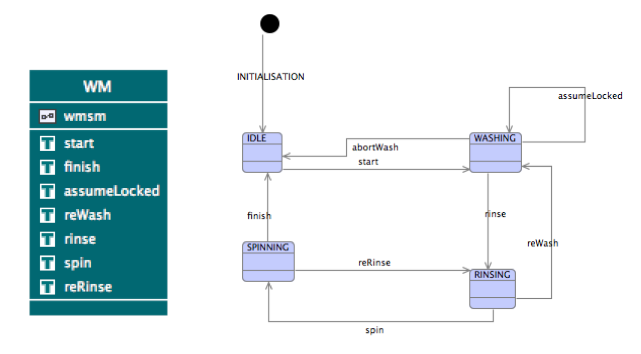
\includegraphics[width=1024]{figures/image13.png}
  \else
  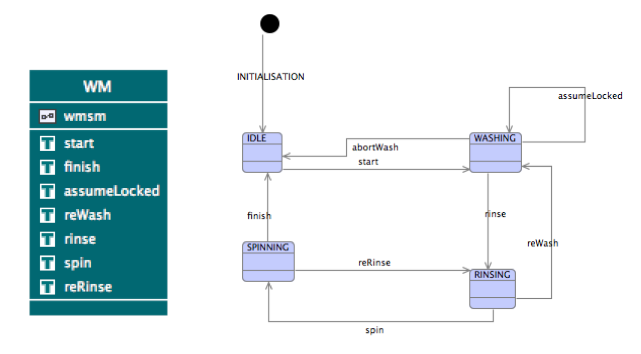
\includegraphics[width=1\textwidth]{figures/image13.png}
  \fi
  \caption{Abstract Model of a Washing Machine}
  \label{fig:AbstractModelOfAWashingMachine}
\end{figure} 

This system-level state machine is untimed and non-deterministic. For instance, when the system is in state RINSING, the system will immediately move to either state SPINNING or WASHING non-deterministically. The state machine represents all the possible mode traces of the system.
Once the state machine has been constructed, the first step is to ensure that all the proof obligations that have been generated by the CODA tool are discharged successfully, as shown in Figure \ref{fig:DischargedProofObligationsOfTheAbstractModel} below. Usually, if the user has added no extra invariants to the model, all the proof obligations should be discharged automatically. If any proof obligations have not been discharged (indicated by an orange question mark icon) they should be examined to determine whether there is a problem with the model. To examine a proof obligation, double click on its icon in the navigator. Switch to the proving perspective by clicking the green tick icon in the right hand corner of the menu bar.  Examine the goal as well as the information tab to work out what the prover is attempting to prove.
 
 \begin{figure}[!htbp]
  \centering
  \ifplastex
  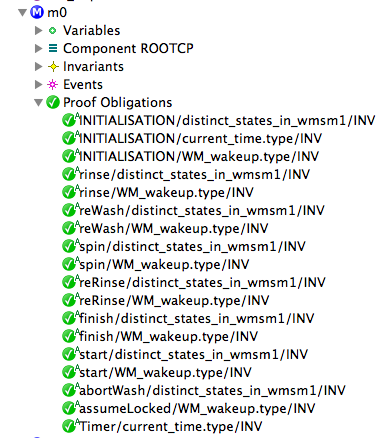
\includegraphics[width=1024]{figures/image14.png}
  \else
  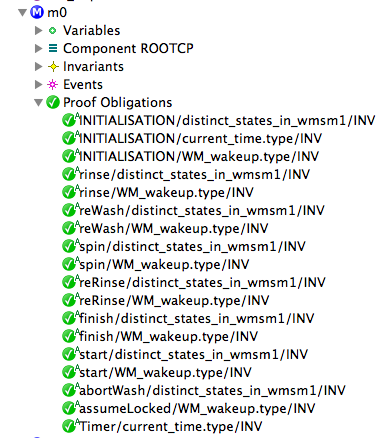
\includegraphics[width=1\textwidth]{figures/image14.png}
  \fi
  \caption{Discharged Proof Obligations of the Abstract Model}
  \label{fig:DischargedProofObligationsOfTheAbstractModel}
\end{figure} 

The next step in the process is to animate the system-level state machine to validate that states and transitions correctly represent the system-level view of the washing machine as shown in Figure \ref{fig:AnimatingTheStatemachineOfTheAbstractModel}. This is a validation process requiring subjective evaluation of the model against system requirements. Does the state-machine behave as desired?

 \begin{figure}[!htbp]
  \centering
  \ifplastex
  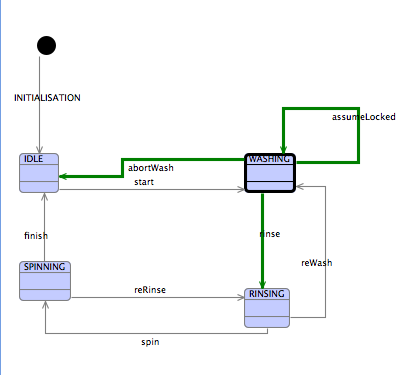
\includegraphics[width=1024]{figures/image15.png}
  \else
  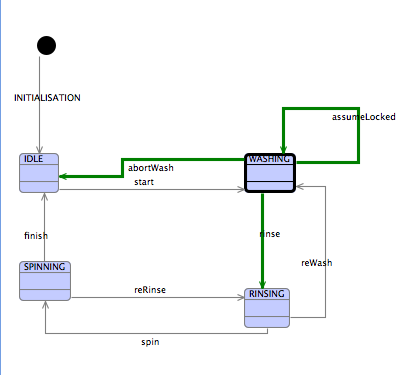
\includegraphics[width=1\textwidth]{figures/image15.png}
  \fi
  \caption{Animating the State-machine of the Abstract Model}
  \label{fig:AnimatingTheStatemachineOfTheAbstractModel}
\end{figure} 

The current state of the system is WASHING, as indicated by the bold, black outline of the state. Three transitions, highlighted in green, are enabled from this state: abortWash, rinse and assumeLocked. Select one from this non-deterministic choice to proceed with the animation. Continue animating the state machine to validate this top-level specification against the system requirements.
The specification may also be validated from the ProB view of Rodin as shown in Figure \ref{fig:AnimatingTheAbstractModelWithProBEventAndHistoryViews} and Figure \ref{fig:AnimatingTheAbstractModelWithProBStateView} below. The event view of Figure  \ref{fig:AnimatingTheAbstractModelWithProBEventAndHistoryViews} presents a list of enabled events from which one may be selected to advance the animation. The history view of Figure  \ref{fig:AnimatingTheAbstractModelWithProBEventAndHistoryViews} shows a record of previous selections. At any stage of the animation it is possible to go back to a selection in the history and perform a new animation from that point.
 
 \begin{figure}[!htbp]
  \centering
  \ifplastex
  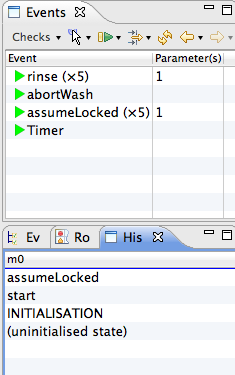
\includegraphics[width=1024]{figures/image16.png}
  \else
  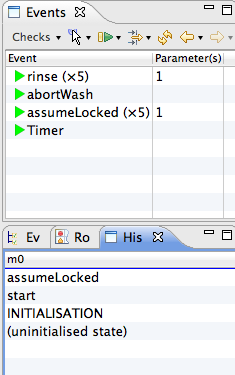
\includegraphics[width=1\textwidth]{figures/image16.png}
  \fi
  \caption{Animating the Abstract Model with ProB Event and History Views}
  \label{fig:AnimatingTheAbstractModelWithProBEventAndHistoryViews}
\end{figure} 

The state view of Figure \ref{fig:AnimatingTheAbstractModelWithProBStateView} shows the current and previous value for each variable. The invariants and guards may also be analysed in this view. The final verification step is to show absence of deadlock using the ProB model checker.

 \begin{figure}[!htbp]
  \centering
  \ifplastex
  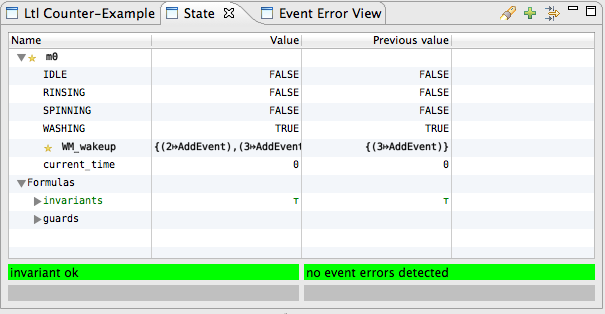
\includegraphics[width=1024]{figures/image17.png}
  \else
  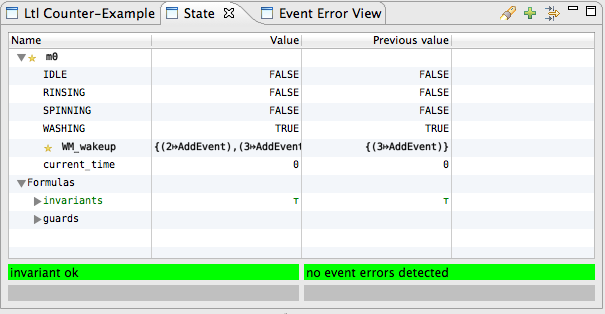
\includegraphics[width=1\textwidth]{figures/image17.png}
  \fi
  \caption{Animating the Abstract Model with ProB State View}
  \label{fig:AnimatingTheAbstractModelWithProBStateView}
\end{figure} 

First the model checker is configured as shown in Figure \ref{fig:ProBModelCheckerOptions} to find deadlocks and invariant violations. For this abstract model, the automatic provers have already proved all the proof obligations, but later in the refinement process it may be more difficult to prove some of the invariants. The model checker can then be used to look for counterexamples that are due to modelling errors. If the model checker reveals a counterexample it is more efficient than embarking on a complex proof that is eventually found to be false. If a counterexample is not revealed (and the complete state space has not been covered) the goal of the proof may still be false. Therefore the goals to be proven should be examined carefully as they often reveal a problem with the model. 
It is important not to leave unproven invariants in a model since if they are not true these could be used in later refinements by the automatic provers to make incorrect deductions.
Selecting symmetry reduction option is not really necessary at this stage, but can help to reduce model checking time when the model is more complex.
When the model checking completes, the results are presented by ProB in the window shown in Figure \ref{fig:ProBModelCheckingCoverageForTheAbstractModel} below.
 
 \begin{figure}[!htbp]
  \centering
  \ifplastex
  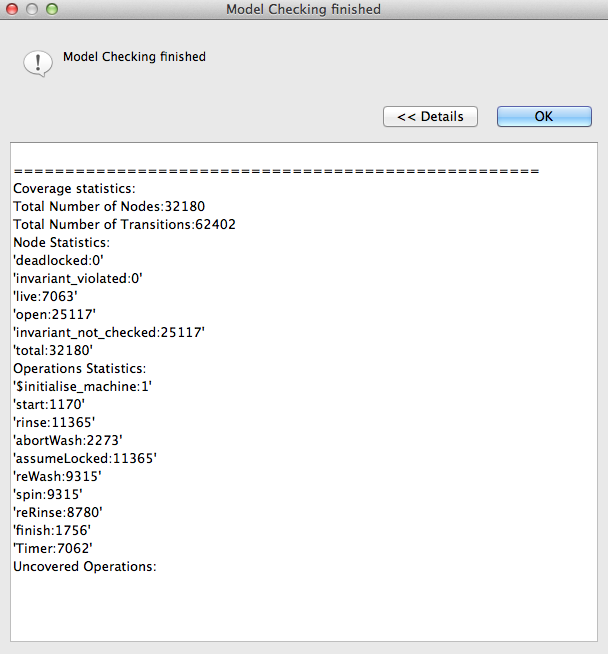
\includegraphics[width=1024]{figures/image18.png}
  \else
  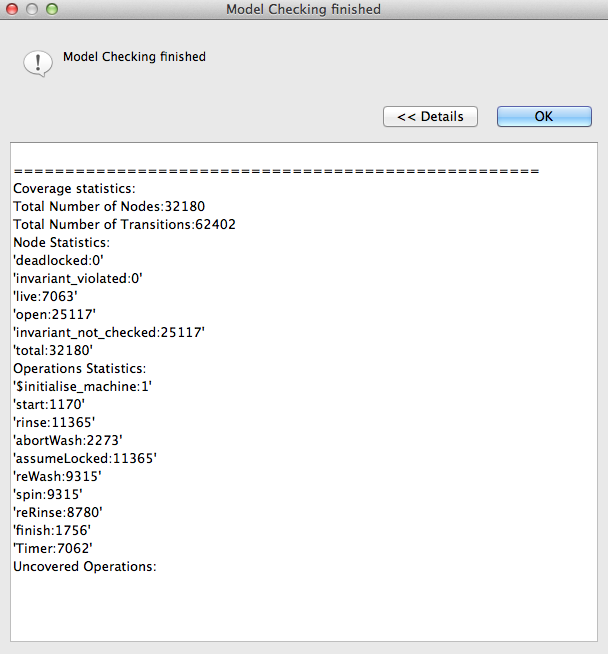
\includegraphics[width=1\textwidth]{figures/image18.png}
  \fi
  \caption{ProB Model Checking Coverage for the Abstract Model}
  \label{fig:ProBModelCheckingCoverageForTheAbstractModel}
\end{figure} 

The interesting coverage metric is shown at the bottom of the window: Uncovered Operations. In this case all operations have been covered which increases confidence in the absence of deadlock.

%%% Local Variables:
%%% mode: latex
%%% TeX-master: "component_diagrams-user_manual"
%%% End:

 \subsection{The First Refinement}
\label{sec:component_diagrams-tutorial_firstRefinement}


The single component and abstract state machine is now refined into a system comprising two components as shown in Figure 20 below. The first component is the Control Panel and the second the abstract washing machine sub-system. Two connectors enable communication between the two components. The first connector, CI, is used to pass the Washing Program ID (PID) to the washing machine sub-system and the second connector, WMSTATE, passes the status of the sub-system back to the Control Panel to be displayed. The state machine is unchanged except for the addition of a self transition on state IDLE which constrains the sendWaiting operation so that it only sends the waiting status over the WMSTATE connector while the washing machine is idle.
 
Figure 20 - First Refinement of Washing Machine

The external operation, UserStart, in component CP represents the user starting the wash by passing the selected wash program, using a port-send action on connector CI to the washing machine sub-system. The port-send action is shown in Figure 21. Note that the minimum delay of 1 is used. The value pid1 is a parameter representing the non-deterministic sending of any PID.
 
Figure 21 - First Refinement : Port Sends on CI

A corresponding port-wake operation, start, in the washing machine sub-system receives the program ID that will, in a subsequent refinement, be decoded to control the wash. The port-wake guard is shown in Figure 22. 
A further port-wake operation, ignoreStart, manages inadvertent start requests from the user. Note that this is necessary due to a design decision not to constrain the sending of start messages from CP. If WM is not in a state to respond to the start an explicit ignoreStart is needed to avoid the system deadlocking.
 
Figure 22 - First Refinement : Port Wakes on CI

When the washing machine sub-system receives the pid, it responds with a port-send action on connector WMSTATE to inform the Control Panel that the washing machine is now RUNNING as shown in Figure 23
 
Figure 23 - First Refinement : Port Sends on WMSTATE

The Control Panel receives the message from the washing machine sub-system with the port-wake operation Running shown in Figure 24 so that this information can be displayed to the washing machine user.
 
Figure 24 - First Refinement : Port Wakes on WMSTATE

The State Machine Animation facility is now used again to validate this 2-component system and the model checker is run to check for deadlocks as shown in Figure 25. Note that, again, all operations have been covered by the model checker.
 
Figure 25 - ProB Model Checking Coverage for the First Refinement


%%% Local Variables:
%%% mode: latex
%%% TeX-master: "component_diagrams-user_manual"
%%% End:

 \subsection{The Second Refinement}
\label{sec:component_diagrams-tutorial_secondRefinement}


The washing machine sub-system component is now further refined, as shown in Figure 26, into two components, the DOOR sub-system and an abstract component, WM, that represents the rest of the washing machine sub-system. Two connectors enable communication between these two components. The first, lock, passes a Boolean signal to the DOOR sub-system to lock the door. The second, doorPosition, informs the Washing Machine sub-system when the door is opened or closed.
 
Figure 26 - Second Refinement of Washing Machine

Note that the DOOR component has two external operations, closeDoor and openDoor, which represent the interaction of the user with the door. Care is needed in this refinement to ensure that the system cannot get into an unsafe state; the door should always be locked when the washing machine is washing, rinsing or spinning so that the user cannot inadvertently open the door and release potentially very hot water.
The state-machine for the washing machine is refined to split the WASHING state into sub-states LOCKINGDOOR and INPROGRESS and IDLE into UNLOCKINGDOOR and IDLEWAITING, Figure 27. This is necessary to accommodate the new transitions concerned with locking and unlocking the door.
 
Figure 27 - Second Refinement : Refined State-machine of the Washing Machine

An invariant, DOORLOCKED  = TRUE, is introduced in the sub-system state machine for states INPROGRESS, RINSING and SPINNING.
The state machine for the door sub-system is shown in Figure 28. The door may be open (DOOROPEN) in which case any instructions to lock the door are ignored (ignoreLock) or it may be closed (DOORCLOSED). When the door is closed it may be unlocked (DOORUNLOCKED) or locked (DOORLOCKED). Note that the transitions unlockDoor and lockDoor are drawn with the superstate DOORCLOSED as their source indicating that they can fire irrespective of whether the door is locked or not.
 
Figure 28 - Second Refinement : State-machine for the Door Component

The washing machine sub-system sends a message via the lock connector to the door sub-system to lock the door if it has received a message from the door via the doorPosition connector indicating that the door is closed.  The washing machine sub-system then initiates a self-wake, delayed by 3 time units, as shown in Figure 29. If the door is still closed at the self-wake, as indicated by the guard 
WM\_doorPosition = CLOSED,  then it is assumed that the door is locked and the system can proceed to the INPROGRESS state. The alternative transition (Figure 27) is abortWash which has the negated guard  WM\_doorPosition $\neq$ CLOSED.
 
Figure 29 - Second Refinement : Self Wake to Check Door Locked

The proof obligations generated for the safety invariant are difficult to discharge. It is a good idea at this stage to proceed immediately to animation and model checking, to ensure that the model behaves as expected.
Model checking does indeed show immediately that the safety invariant is violated and provides a counterexample in the history pane as shown in Figure 30.
 
Figure 30 - Counterexample Discovered by ProB

Although the refinement models the latency that certainly exists between the washing machine sub-system and door sub-system, it allows the user to open and close the door repeatedly in zero-time. Modelling this Zeno Behaviour is unrealistic and results in a scenario where the user can close the door and then open it again immediately just before it is locked.
The solution is to model more realistically the latency that must exist in the opening and closing of the door by introducing a delay on the External Event, closeDoor, as shown in Figure 31. The guard  \textbf{\code{current\_time > DOOR\_latency}}, where DOOR\_latency is a variable that is set to current\_time + 1 by any preceding door open or close events, ensures that two door events cannot occur on consecutive clock ticks. This corresponds to an assumption that the systems time response makes it impossible to open and close the door without it being detected. This is sufficient to ensure that any changes of door state are successfully transmitted to the WM component.
 
Figure 31 - Introducing Latency to the Door Operations
 
The model checker is re-run to verify that the invariant violation has been addressed and that there is no deadlock, as shown in Figure 32. Note now, that the model checking results show that not all operations have been covered, though examination of the guards and actions of these uncovered operations show that none are material to the invariant violation being investigated. Although not a proof, model checking with operation coverage gives confidence that the model is behaving as expected.
 
Figure 32 - ProB Model Checking Coverage for the Second Refinement 
 
To improve operation coverage, it is a good idea to try the alternative Breadth First Search option. Figure 33 shows the improved coverage results and Figure 34 shows how this option is set.
 
Figure 33 - ProB Model Checking Coverage for the Second Refinement : Breadth First
 
Figure 34 - Configuration for ProB Model Checker Breadth First Option
 
%%% Local Variables:
%%% mode: latex
%%% TeX-master: "component_diagrams-user_manual"
%%% End:

 \subsection{The Third Refinement}
\label{sec:component_diagrams-tutorial_thirdRefinement}
 
Now we refine the notion of the Program. We associate with each PID a washTime, rinseTime and spinTime and also introduce a WashCount and SpinCount as shown in Figure 35. These properties constrain and make deterministic the operation of the washing machine sub-system for a given PID.
 
Figure 35 - Adding Wash Program Details to the Model
 
The delay introduced for each wash mode is modelled using a SelfWake as shown for the rinse mode in Figure 36.
 
Figure 36 - Introducing Wash Program Delays using Self Wakes
 
The number of washes or rinses associated with a program is modelled using a counter which is decremented and hence completes at rinseCounter = 0, as shown in Figure 37.
 
Figure 37 - Introducing Wash Program Cycles using Guards
 
Again, the model checker is run to verify that no deadlocks have been introduced into the system. Since this refinement is only to strengthen the guards, invariant preservation is not an issue in this refinement. Note that as shown in Figure 38, full operation coverage is achieved. The program constraints introduced in this refinement have reduced the model state space. 
 
Figure 38 - ProB Model Checking Coverage for the Third Refinement
 
The state machine is shown in Figure 39 below. Invariants concerning the counters have been added to the INPROGRESS and RINSING states. These invariants help ensure that no mistakes have been made in constructing the counters.
 
Figure 39 - State-machine for the Third Refinement 
 

%%% Local Variables:
%%% mode: latex
%%% TeX-master: "component_diagrams-user_manual"
%%% End:

 \subsection{The Fourth Refinement}
\label{sec:component_diagrams-tutorial_fourthRefinement}

 
The washing machine sub-system is now further partitioned into 2 components: the drum sub-system and an abstract component representing the remaining washing machine sub-system, following the pattern of previous refinements.
The component diagram is shown in Figure \ref{fig:FourthRefinementOfWashingMachine}.
Three boolean connectors pass messages from the washing machine sub-system to the drum to open and close the hot or cold water valves and to switch the drain pump on or off. Two further natural number connectors pass the water level and the water temperature back from the drum to the washing machine sub-system.
 
 \begin{figure}[!htbp]
  \centering
  \ifplastex
  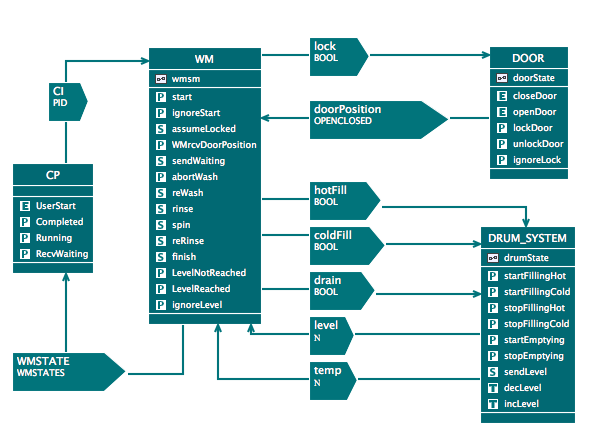
\includegraphics[width=1024]{figures/image41.png}
  \else
  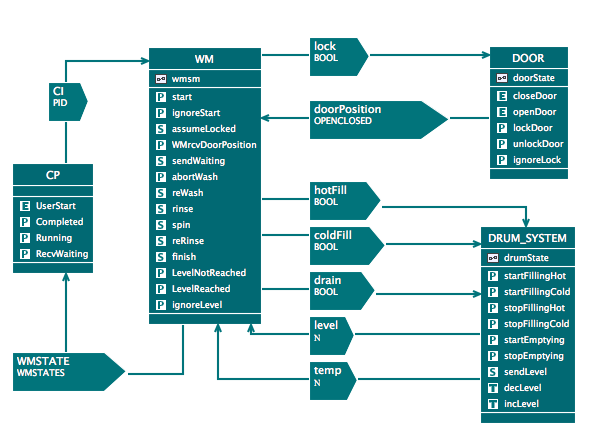
\includegraphics[width=1\textwidth]{figures/image41.png}
  \fi
  \caption{Fourth Refinement of Washing Machine}
  \label{fig:FourthRefinementOfWashingMachine}
\end{figure} 
 
The state machine for the drum sub-system is shown in Figure \ref{fig:FourthRefinementStatemachineForTheDrumComponent}.
 
 \begin{figure}[!htbp]
  \centering
  \ifplastex
  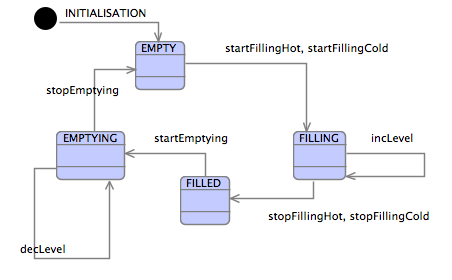
\includegraphics[width=1024]{figures/image42.png}
  \else
  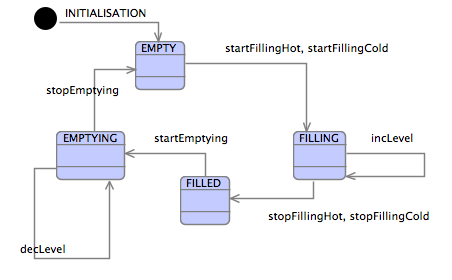
\includegraphics[width=1\textwidth]{figures/image42.png}
  \fi
  \caption{Fourth Refinement : State-machine for the Drum Component}
  \label{fig:FourthRefinementStatemachineForTheDrumComponent}
\end{figure} 
 
The washing machine state machine is now further refined to manage the filling and emptying of the drum by monitoring the water level as shown in Figure \ref{fig:FourthRefinementRefinedStatemachineOfTheWashingMachine}.
 
 \begin{figure}[!htbp]
  \centering
  \ifplastex
  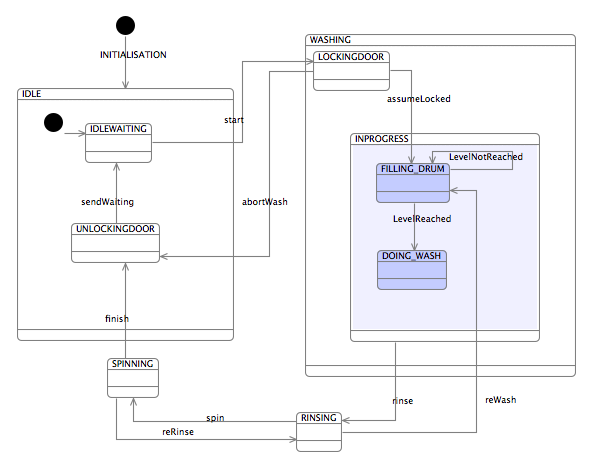
\includegraphics[width=1024]{figures/image43.png}
  \else
  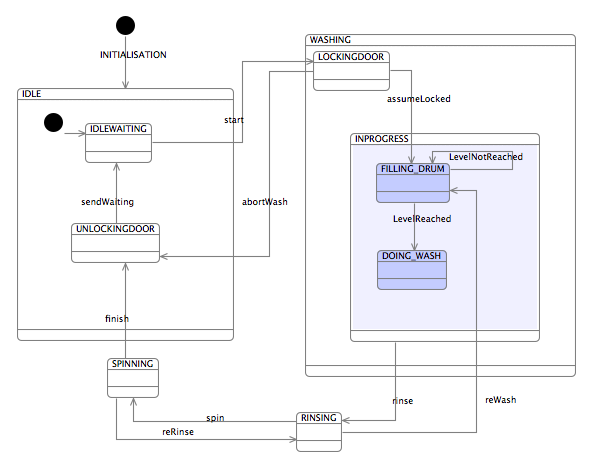
\includegraphics[width=1\textwidth]{figures/image43.png}
  \fi
  \caption{Fourth Refinement : Refined State-machine of the Washing Machine}
  \label{fig:FourthRefinementRefinedStatemachineOfTheWashingMachine}
\end{figure}  
 
The value TRUE is sent on the coldFill connector as shown in Figure \ref{fig:FourthRefinementPortSendOnTheColdFillConnector}.
 
 \begin{figure}[!htbp]
  \centering
  \ifplastex
  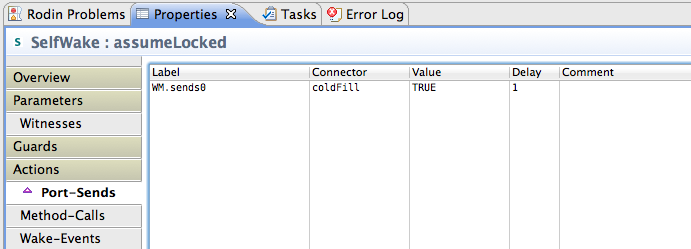
\includegraphics[width=1024]{figures/image44.png}
  \else
  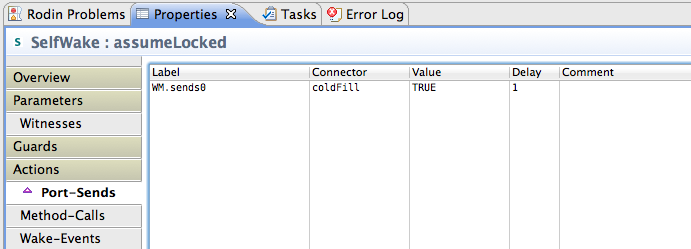
\includegraphics[width=1\textwidth]{figures/image44.png}
  \fi
  \caption{Fourth Refinement : Port Send on the coldFill Connector}
  \label{fig:FourthRefinementPortSendOnTheColdFillConnector}
\end{figure} 
 
The drum sub-system receives the value on the coldFill connector and starts filling the drum (Figure \ref{fig:FourthRefinementPortWakeOnTheColdFillConnector}).
 
 \begin{figure}[!htbp]
  \centering
  \ifplastex
  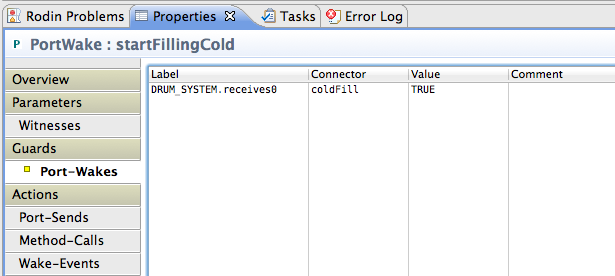
\includegraphics[width=1024]{figures/image45.png}
  \else
  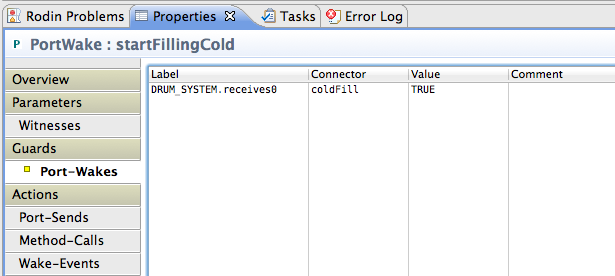
\includegraphics[width=1\textwidth]{figures/image45.png}
  \fi
  \caption{Fourth Refinement : Port Wake on the coldFill Connector}
  \label{fig:FourthRefinementPortWakeOnTheColdFillConnector}
\end{figure}  
 
The drum sub-system sends the value of water level and water temperature repeatedly at unit delay intervals using the self-wake operation sendLevel of Figure \ref{fig:FourthRefinementSelfWakeToRepeatedlySendOnLevelAndTempConnectors}.
 
 \begin{figure}[!htbp]
  \centering
  \ifplastex
  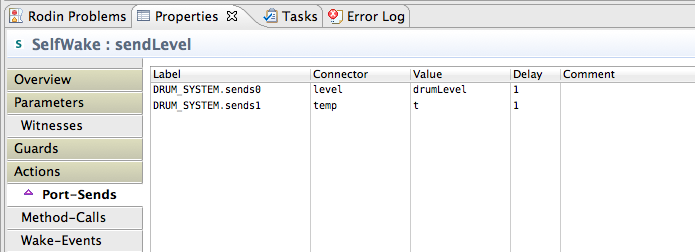
\includegraphics[width=1024]{figures/image46.png}
  \else
  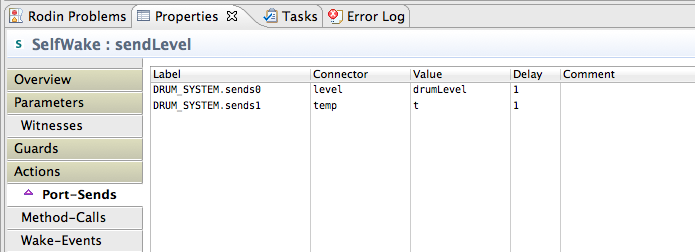
\includegraphics[width=1\textwidth]{figures/image46.png}
  \fi
  \caption{Fourth Refinement : Self Wake to Repeatedly Send on level and temp Connectors}
  \label{fig:FourthRefinementSelfWakeToRepeatedlySendOnLevelAndTempConnectors}
\end{figure} 
 
The washing machine sub-system switches off the water valve when it detects that the water level associated with the PID has been reached, as shown in Figure \ref{fig:FourthRefinementGuardedPortWakeToRespondWhenLevelReached}.
 
 \begin{figure}[!htbp]
  \centering
  \ifplastex
  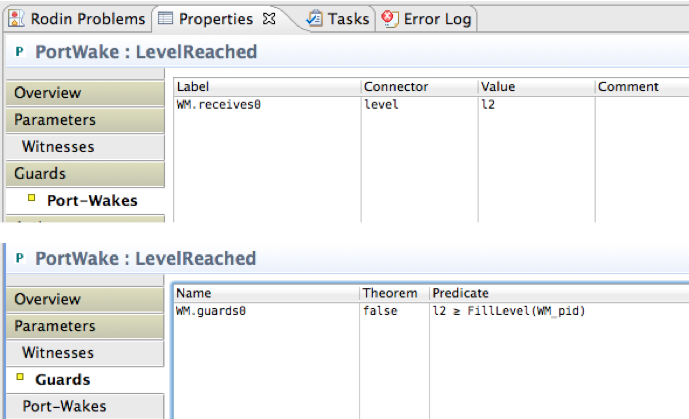
\includegraphics[width=1024]{figures/image47.png}
  \else
  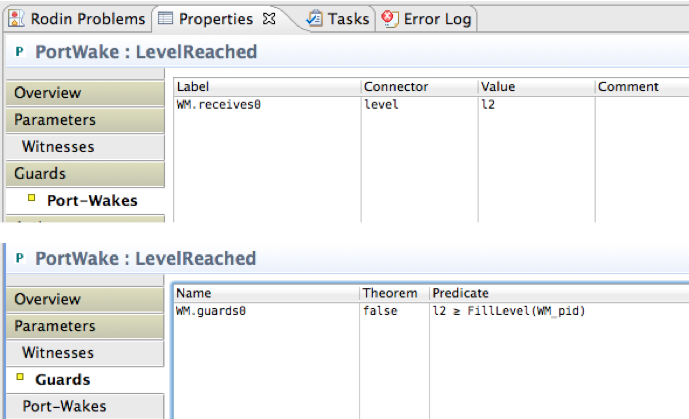
\includegraphics[width=1\textwidth]{figures/image47.png}
  \fi
  \caption{Fourth Refinement : Guarded Port Wake to Respond when Level Reached}
  \label{fig:FourthRefinementGuardedPortWakeToRespondWhenLevelReached}
\end{figure}  
 
The model checker is run again to show absence of deadlock. Note that because of the added complexity of this refinement, not all operations are covered (Figure \ref{fig:ProBModelCheckingCoverageForTheFourthRefinement}). Sufficient operations, however, have been covered to give confidence that filling operation is performing satisfactorily.
 
 \begin{figure}[!htbp]
  \centering
  \ifplastex
  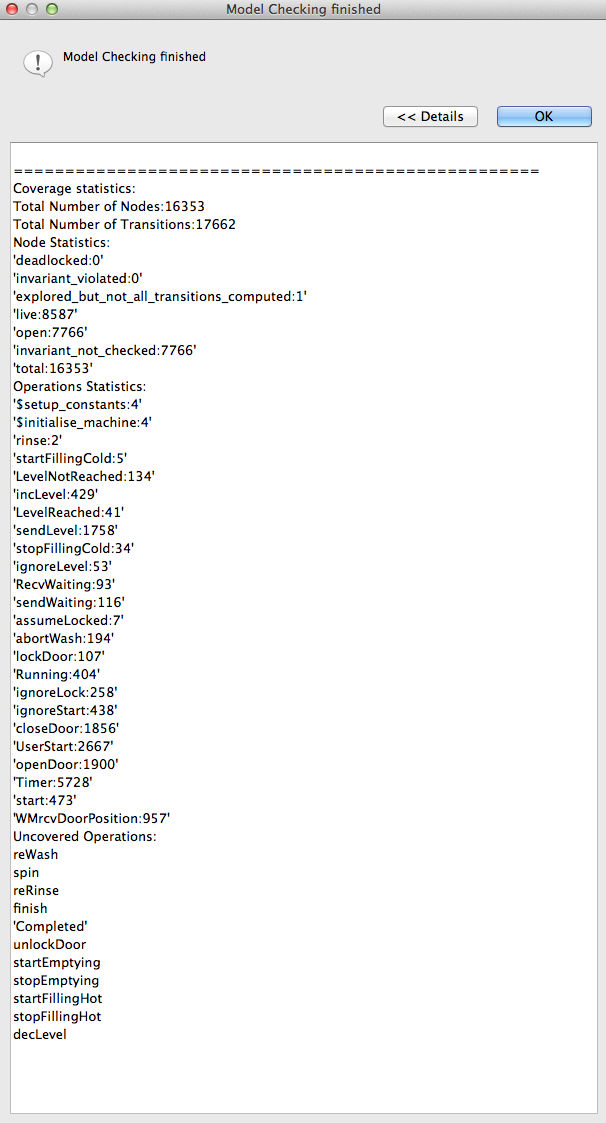
\includegraphics[width=1024]{figures/image48.png}
  \else
  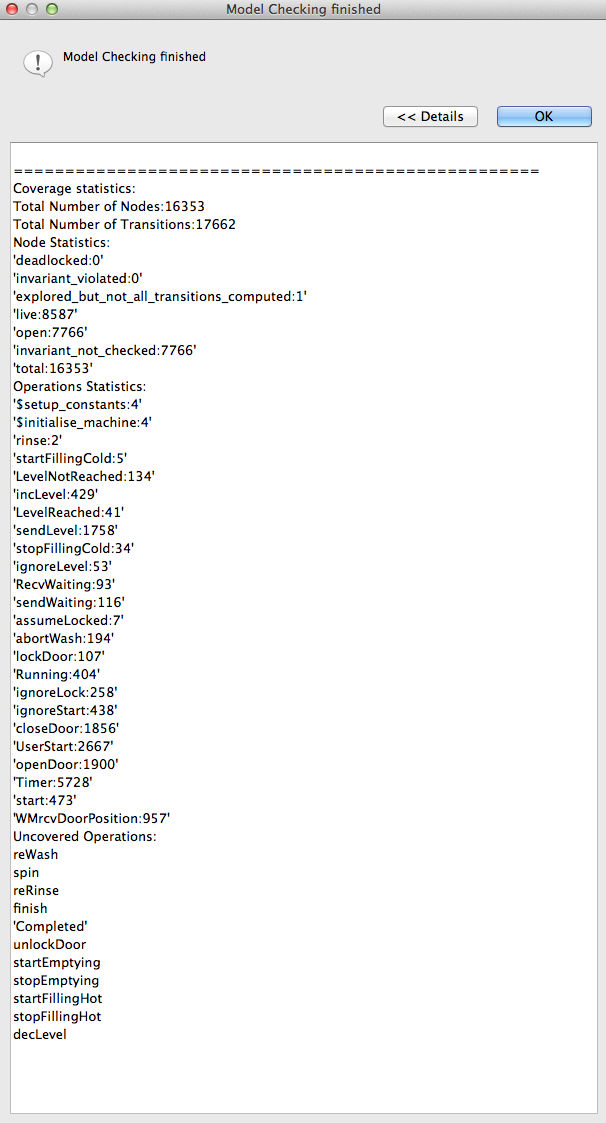
\includegraphics[width=1\textwidth]{figures/image48.png}
  \fi
  \caption{ProB Model Checking Coverage for the Fourth Refinement}
  \label{fig:ProBModelCheckingCoverageForTheFourthRefinement}
\end{figure}  


%%% Local Variables:
%%% mode: latex
%%% TeX-master: "component_diagrams-user_manual"
%%% End:

 
\subsection{Further Refinements}
 
The refinement strategy that has been established in the earlier refinements can continue as the agitator motor and heater components are introduced. At each stage the abstract washing machine sub-system component is constrained until it finally represents just the
  hardware/software controller
   that is being developed for the washing machine.
 
\subsection{Running the Oracle Simulator}
 
The CODA simulator can be used at every refinement step to establish a set of regression tests and golden results. Figure 48 illustrates the state of the system at times 10, 14, 15 and 18.

Figure 48 - Snapshots of CODA Simulator at Times 10, 14, 15 and 18
 
\subsection{Conclusion}
 
A method for system modelling and refinement has been illustrated using the washing machine case study example. Modelling begins with an abstract state machine model of the system, which is systematically refined into a set of communicating processes - the hardware/software controller under development and the components that represent the controller environment.
At each refinement step, formal proof and model checking is used to validate the model against the requirements and to show absence of deadlock.
The final hardware/software controller component can then be verified within a component-based environment using the CODA Oracle Simulator.

%%% Local Variables:
%%% mode: latex
%%% TeX-master: "component_diagrams-user_manual"
%%% End:
